\documentclass[acmlarge]{acmart}

\usepackage{booktabs} % For formal tables


\usepackage[ruled]{algorithm2e} % For algorithms
\renewcommand{\algorithmcfname}{ALGORITHM}
\SetAlFnt{\small}
\SetAlCapFnt{\small}
\SetAlCapNameFnt{\small}
\SetAlCapHSkip{0pt}
\IncMargin{-\parindent}
\newcommand{\Mod}[1]{\ (\mathrm{mod}\ #1)}
<<<<<<< HEAD

=======
>>>>>>> 0558b482e5cd7a38552115660d4d327b7d375ccc
% Metadata Information
%\acmJournal{PACMHCI}
%\acmVolume{9}
%\acmNumber{4}
%\acmArticle{39}
%\acmYear{2010}
%\acmMonth{3}
%\acmArticleSeq{11}


% DOI
\acmDOI{0000001.0000001}

% Paper history
%\received{February 2007}
%\received{March 2009}
%\received[accepted]{June 2009}


% Document starts
\begin{document}
% Title portion
\title{Security Suite: EECS 444 Final Project}
% \titlenote{We can add a note to the title}

\author{Kim Almcrantz}
\affiliation{\institution{Destroyer of Worlds}}
\email{kaa97@case.edu}

\author{Mark Lalor}
\affiliation{\institution{Eater of Nightmares}}
\email{mwl58@case.edu}

\author{Brian Li}
\affiliation{\institution{Summoner of Flames}}
\email{bvl8@case.edu}

\author{Vanessa Melikian}
\affiliation{\institution{Reaper of Souls}}
\email{vlm21@case.edu}

\author{Maya Nayak}
\affiliation{\institution{Tormentor of the Lost}}
\email{mkn30@case.edu}

\author{Jacob Wise}
\affiliation{\institution{Annihilator of the Innocent}}
\email{jsw107@case.edu}


%\begin{abstract}
%This is our abstract. Currently it is empty because no one has written it. In order to make it not empty, it must be written/
%\end{abstract}

\keywords{encryption, cipher, hash, entropy}

\maketitle

% The default list of authors is too long for headers.
% \renewcommand{\shortauthors}{G. Zhou et al.}

\section{Abstract}

This is our abstract. Currently it is empty because no one has written it. In order to make it not empty, it must be written.

\section{Introduction}\label{sec:intro}

Modern communications require special methods to ensure the security of information in the presence of adversaries that want to intercept or maliciously modify communicated data. An adversary may try to compromise the confidentiality, or integrity of data, or they may bypass an authentication completely with a carefully-crafted message.

Symmetric key ciphers

To begin, we ponder a quote from an anonymous philosopher.
\begin{quote}
  ``where's brian ''.
\end{quote}}}
What does it mean? Who said it? Why was it said? We may never know. But what we do know is the following:

This article is divided into several sections, in Section [\ref{sec:intro}], we introduce the cryptographic environment that we will explore. In Section [\ref{sec:algorithms}] we describe implementations of several symmetric and asymmetric encryption algorithms, and then Section [\ref{sec:gui}] we present our tool \textsc{SecuritySuiteGUI}, a software suite to experiment with these implementations. We then demonstrate the power of password cracking with a hashcat demo in Section [\ref{sec:hashcat}]. Finally, we demonstrate how the Vigenère cipher may be easily cracked with computational power in Section [\ref{sec:vinegar}]. We evaluate our methods in Section [\ref{sec:evaluation}], and then discuss our techniques, challenges, and other thoughts in Section [\ref{sec:discussion}]. Finally, we discuss our final conclusions in Section [\ref{sec:conclusions}].

% itemize
\begin{itemize}
\item To the best of our knowledge, this is not the first time something like this was developed
\item We use \cite{Adya-01}, for a chocolate chip cookie recipe.
\end{itemize}

\subsection{Basic Crypto Stuff}

This is a talk about all the types of ciphers, symmetric, asymmetric, maybe more!

\section{Tool Design} \label{sec:impl}
\subsection{Algorithm Implementations} \label{sec:algorithms}

\subsubsection{DES}

We show a high-level implementation of DES in Algorithm \ref{alg:des}. The DES algorithm has X main steps:

\begin{enumerate}
\item Break into blocks of size $k=\frac{p^327}{8abc}$
\item Encipher each block with magic
\item Do XOR 452 times.
\end{enumerate}


% Algorithm
\begin{algorithm}[t]
\label{rsa_algo}
\SetAlgoNoLine
\KwIn{Public key exponent $e$, key size $s$}
\KwOut{Public key $k_{pub}$, and private key $k_{priv}$}

\Repeat{$\gcd(e, \lambda) = 1 \land \|p - q\| \geq 2^{s / 2 - 100}$}{
    $p \longleftarrow \text{probable-prime}(s / 2)$

    $q \longleftarrow \text{probable-prime}(s / 2)$

    $\lambda \longleftarrow \text{lcm}(p - 1, q - 1)$
}

$k_{pub} \longleftarrow pq$

$k_{priv} \longleftarrow e^{-1} \mod{\lambda}$

\KwRet $k_{pub}$, $k_{priv}$
\caption{RSA Keygen implementation}
\label{alg:rsa-keygen}
\end{algorithm}

\subsubsection{RSA}
\hspace*{\fill} \\ % force newline
Unlike DES and Vignere, RSA is an asymmetric cipher. Specifically, this means that the RSA cipher (i.e. public key) used to encrypt a message cannot be used to decrypt the the encrypted message whereas the cipher used to encrypt a message in DES and Vignere can be used to decrypt the encrypted message by reversing the encryption process.
		
To use RSA, a user first generates a key pair. The key pair contains a private key, public key, and a public key exponent. The public key and public key exponent can be made public so that other users can send the original user an encrypted message. The original user can use his/her private key to messages encrypted with the published public key and exponent. The main benefit that asymmetric encryption provides is that communicating entities can securely communicate without exchanging a decryption key/cipher.

The key mechanic in RSA comes from the following congruence:

\begin{equation}
\label{rsa_mechanic}
	m^{ed} \equiv m \Mod{pq}
\end{equation}

When ed satisfies:

\begin{equation}
\label{ed_equiv}
	ed \equiv 1 \Mod{\lambda(pq)}
\end{equation}
\begin{equation}
\label{carmichael}
	\lambda(pq) = lcm(p - 1, q - 1)
\end{equation}

To see why \ref{rsa_mechanic} is true, we will give a proof:
\begin{equation}
\begin{split}
	m^{ed} 
	\equiv m^{k\lambda(pq) + 1} \Mod{pq} \\
	\equiv m * m^{k\lambda(pq)} \Mod{pq} \\
	\equiv m * (m^{\lambda(pq)})^{k} \Mod{pq} \\
	\equiv m * (1)^{k} \Mod{pq} \\
	\equiv m
\end{split}
\end{equation}

To get:
\begin{equation}
	m * (m^{\lambda(pq)})^{k} \Mod{pq} \equiv m * (1)^{k} \Mod{pq}
\end{equation}

We use the Carmichael theorem which gives us the congruence:
\begin{equation}
	a^{\lambda(n)} \equiv 1 \Mod{n}
\end{equation}

Using \ref{rsa_mechanic}, we can let e, d, and n be public key exponent, private key, and public key respectively. If m is the message, we can encrypt messages with the public key and public key exponent by:

\begin{equation}
	m^{e} \equiv c \Mod{n}
\end{equation}

Where c is the encrypted message. Then, we can decrypt messages with the public key and private key by:

\begin{equation}
	c^{d} \equiv (m^{e})^{d} \equiv m^{ed} \equiv m \Mod{n}
\end{equation}

Now that we have shown the correctness of RSA, we will now discuss the algorithm to generate a key pair consisting of a public key exponent, public key, and private key. Algorithm \ref{rsa_algo} gives pseudocode for generating an RSA key pair. Specifically, two large, random numbers are generated. Since it is not computationally feasible to check if the generated numbers are prime with certainty, Miller-Rabin is used to determine if the generated numbers are prime with a certain probability (citation needed). The more rounds of Miller-Rabin a number passes, the more likely the number is prime (citation needed). In Java's BigInteger class, the probablePrime() function returns a prime with probability $1 - 2^-100$ (citation needed). After generating two probable prime numbers, p and q, we ensure that e and $\lambda$ are co-prime and that p and q are at least a few magnitudes apart to make factorizing pq more difficult (citation needed). Finally, we return pq as the public key, e as the public key exponent, and $e^{-1} \Mod{pq}$ as the private key.

%RSA Citations:
%https://docs.oracle.com/javase/7/docs/api/java/math/BigInteger.html#probablePrime(int,%20java.util.Random)
%http://hg.openjdk.java.net/jdk8/jdk8/jdk/file/tip/src/share/classes/java/math/BigInteger.java
%Rivest, R.; Shamir, A.; Adleman, L. (February 1978). "A Method for Obtaining Digital Signatures and Public-Key Cryptosystems" (PDF). Communications of the ACM. 21 (2): 120–126. doi:10.1145/359340.359342. 
% The above citation is used for why the primes need to be a certain distance apart.

\subsubsection{Vigenère Cipher}
\hspace*{\fill} \\ % force newline
\textit{TODO: Vigenère Cipher Description}

\subsection{SecuritySuiteGUI}\label{sec:gui}

% Figure
\begin{figure}
  \centering
  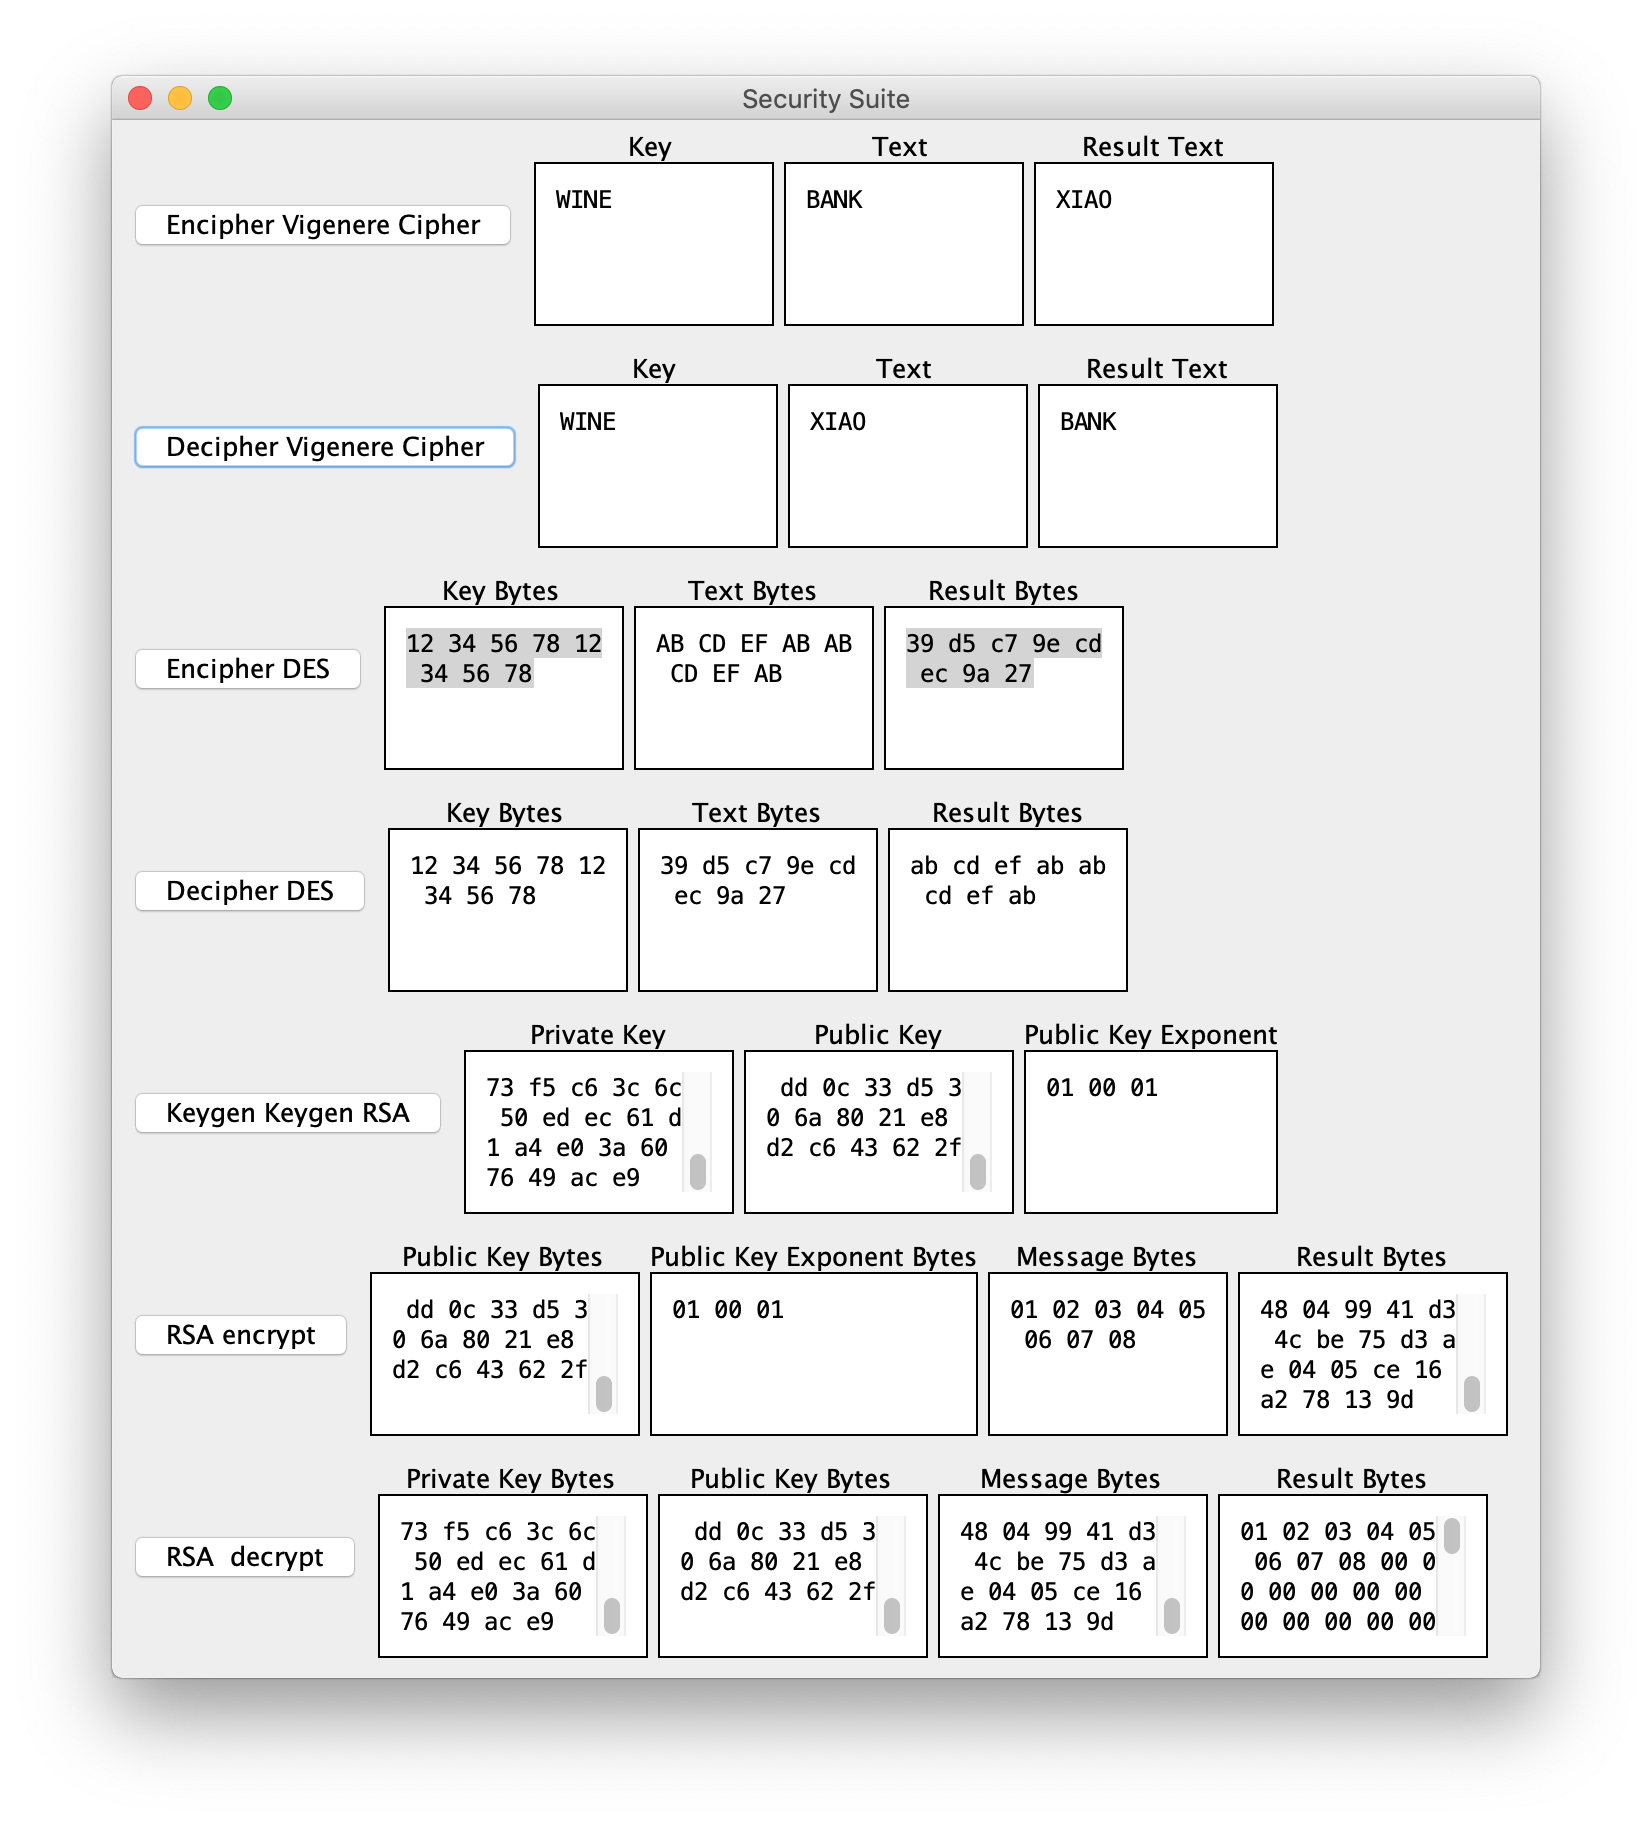
\includegraphics[scale=0.40]{demo}
  \Description{Image of our demo tool}
  \caption{Image of the security suite demo tool.}
  \label{fig:one}
\end{figure}

\subsection{Hashcat Demo}\label{sec:hashcat}

\textsc{Hashcat} is a software tool used to crack passwords by leveraging the highly-parallelized general purpose computation capabilities of GPU \cite{Hashcat}. \textsc{Hashcat} will calculate hashes based on one of several attack modes, and the hashes are automatically checked against the hashes selected to be attacked.

The most important option when using \textsc{Hashcat} is the \texttt{hash-type}, which specifies the actual hash algorithm that will be used for the attack. For example, you can choose a simple hash algorithm such as \texttt{"md5"}, or you may choose a composition of algorithms such as \texttt{"sha1(\$salt.sha1(\$pass))"}.

Depending on the algorithm, \textsc{Hashcat} may or may not be able to leverage the GPU's capabilities effectively. Some algorithms, such as \texttt{bcrypt} are specifically designed to be difficult to parallelize in GPU hardware. Despite having thousands of cores to parallel computation, the algorithm is bottlenecked by the shared memory bus since the algorithm requires operating on a shared block of memory. Other algorithms, such as \texttt{MD5} are able to be run on the order of \textit{trillions} of time per second on modern hardware setups.

The second required option is an \texttt{attack mode}. The simplest is a \texttt{brute-force attack}, which tries all possible combinations in a given keyspace. For example, a brute-force attack may be done on the following charset:

\begin{center}
\texttt{abcdefghijklmnopqrstuvwxyz0123456789}	
\end{center}

If we use this in conjunction with a password length of $6$, this will try all passwords composed of $6$ characters from that charset. For example, the password \texttt{k39a1j} will be discovered this way.

When trying to crack many passwords, the simple \texttt{brute-force attack} is usually an unrealistic attack method. The \texttt{mask attack} can use multiple charsets and string patterns to reduce the password candidate keyspace. 

\section{Vigenère Cipher Cracker}\label{sec:vinegar}

Words go here too!

\section{Results}\label{sec:results}

Evaluation, efficiency? Challenges?

\section{Related Work}\label{sec:relatedwork}

Related work. Examples of citations with DOIs: \cite{2004:ITE:1009386.1010128, Kirschmer:2010:AEI:1958016.1958018}. Online citations: \cite{TUGInstmem, Thornburg01, CTANacmart}.

\section{Discussion}\label{sec:discussion}

What didn't we cover? :O

% Appendix
\appendix
\section{Elaboration on the ABCD algorithm}

This is an appendix, maybe about some equation
\begin{displaymath}
P=NP
\end{displaymath}

\section{Supplementary Materials}

\subsection{Hashcat materials}

Materials?

\subsection{Tool: Symmetric Ciphers Online }

\href{http://symmetric-ciphers.online-domain-tools.com/}{Link}

\begin{acks}

The authors would like to thank the mitochondria for being the powerhouse of the cell.

\end{acks}

% Bibliography
\bibliographystyle{ACM-Reference-Format}
\bibliography{bibliography}

\end{document}
